\documentclass{beamer}

\usepackage[utf8]{inputenc}
\usepackage{hyperref}

\usetheme{Berkeley}
\beamertemplatenavigationsymbolsempty
\setbeamertemplate{headline}{}
 
\title{Importing data into FoodChain-Lab 1}
\date{}
 
\begin{document}
\maketitle

\section{ }

\subsection{Tasks}
\begin{frame}
	\begin{itemize}
		\item In this tutorial we show you how import delivery data to FoodChain-Lab via our Excel templates.
		\item We will first import the inital data for the outbreak locations and the successively add the delivery data for caterers and other suppliers via auto-generated back- and forward-tracing templates.
		\item In FoodChain-Lab it is also possible to import the whole delivery network from one Excel file, but procedure is not documented here. The "All In One" template can be downloaded from here: \url{https://github.com/SiLeBAT/BfROpenLabResources/raw/master/GitHubPages/templates/All_In_One_Template.xlsx}.
	\end{itemize}
\end{frame}
 
\subsection{1}
\begin{frame}
	\begin{center}
  		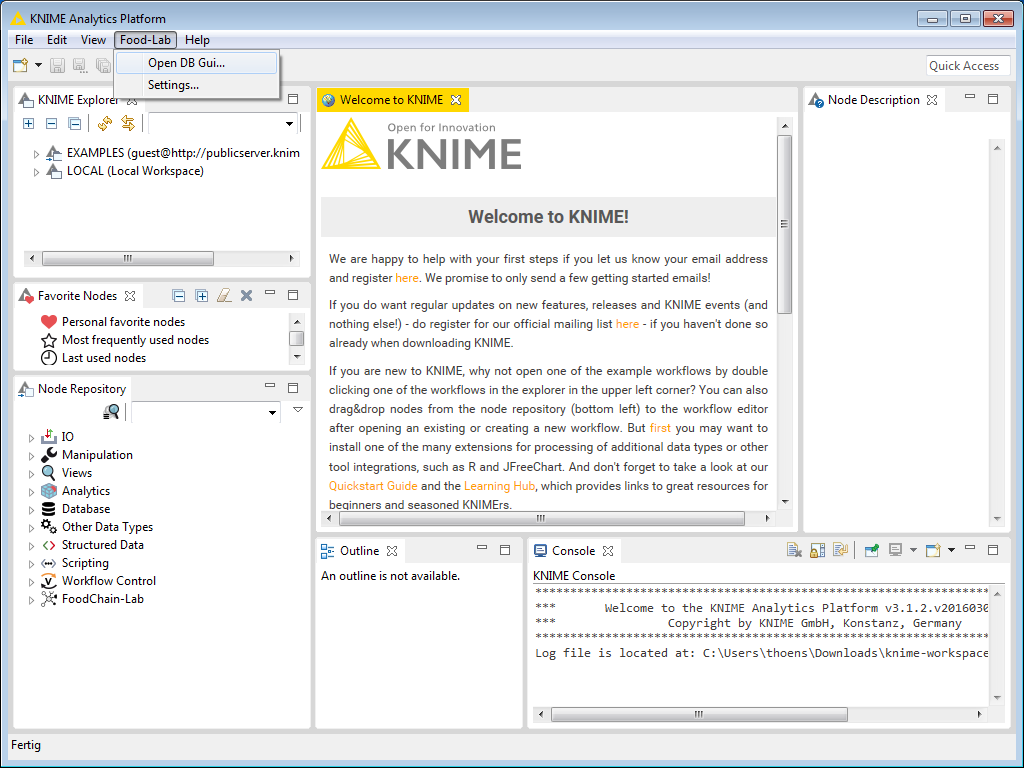
\includegraphics[height=0.6\textheight]{1.png}
	\end{center}
	\begin{itemize}
		\item Select \textbf{Food-Lab $>$ Open DB Gui...} in the menu bar to open the database dialog.
	\end{itemize}
\end{frame}

\subsection{2}
\begin{frame}
	\begin{center}
  		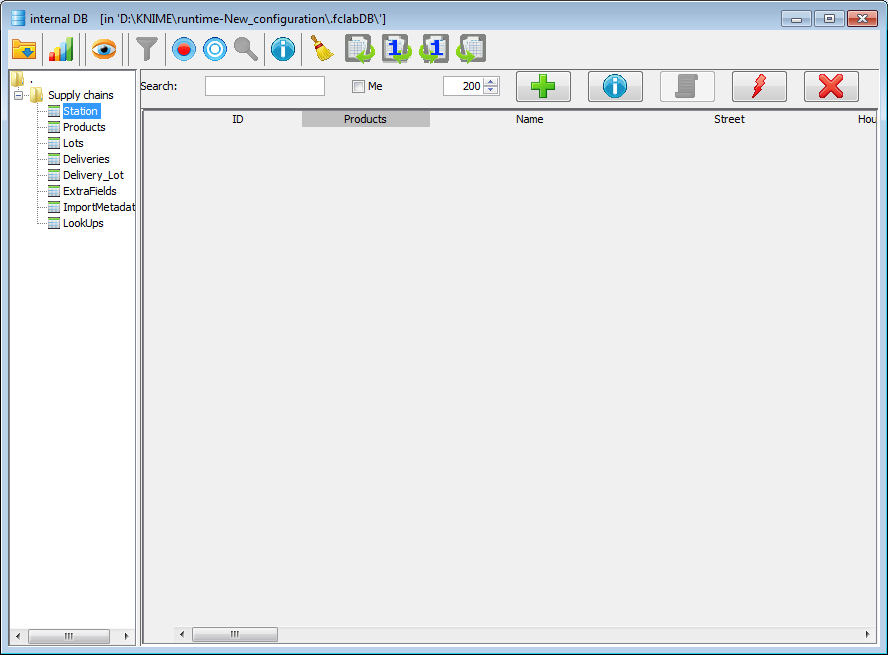
\includegraphics[height=0.5\textheight]{2.png}
	\end{center}
	\begin{itemize}
		\item The FoodChain-Lab database dialog should not pop up.
		\item Here you can import, edit and validate food delivery data.
		\item To start the data import you must download, fill out and import the "Start Tracing Template".
		\item It can be downloaded from here: \url{https://github.com/SiLeBAT/BfROpenLabResources/raw/master/GitHubPages/templates/Start_Tracing_Template.xlsx}.
	\end{itemize}
\end{frame}

\subsection{3}
\begin{frame}
	\begin{center}
  		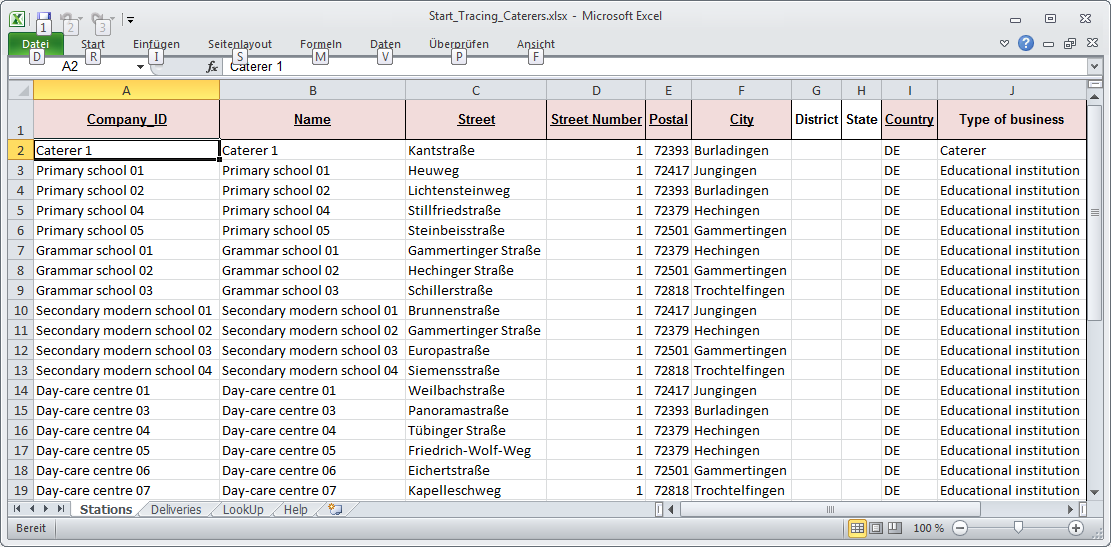
\includegraphics[width=0.95\textwidth]{3.png}
	\end{center}
	\begin{itemize}
		\item
	\end{itemize}
\end{frame}

\subsection{4}
\begin{frame}
	\begin{center}
  		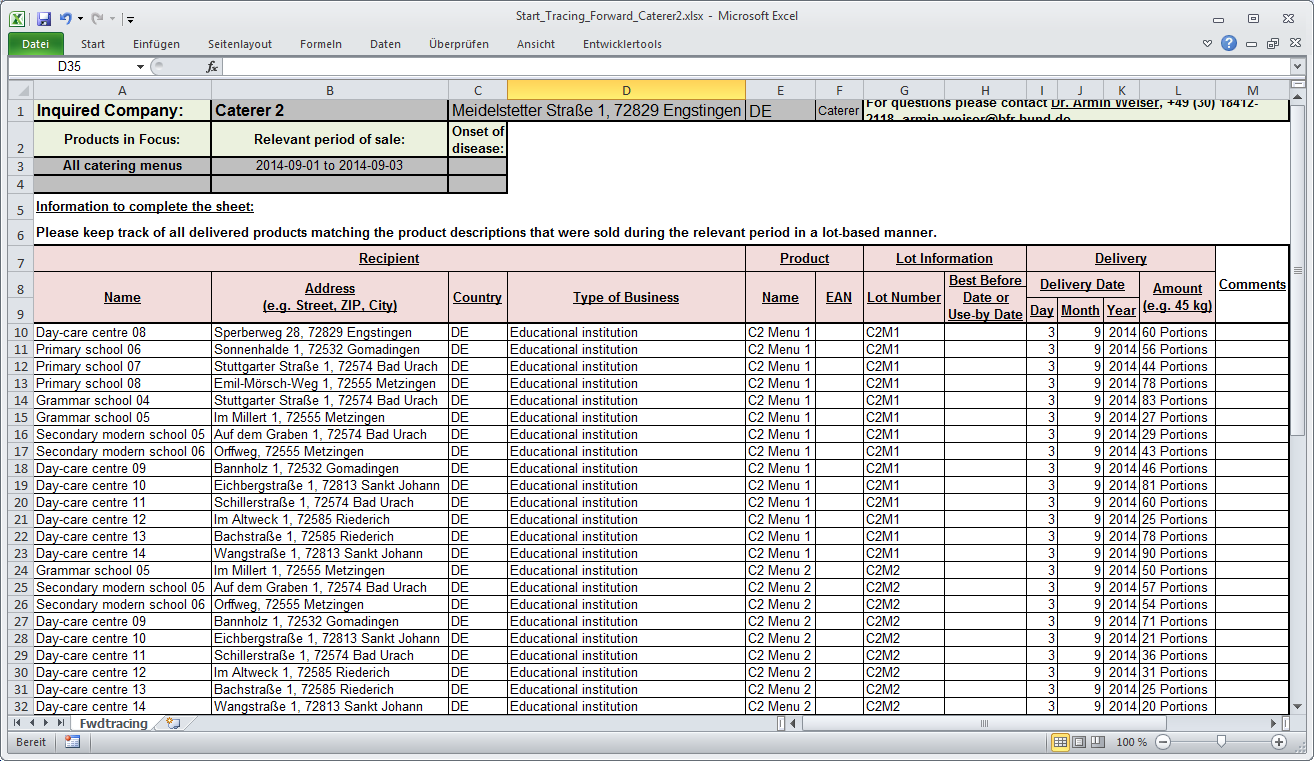
\includegraphics[width=0.95\textwidth]{4.png}
	\end{center}
	\begin{itemize}
		\item
	\end{itemize}
\end{frame}

\subsection{5}
\begin{frame}
	\begin{center}
  		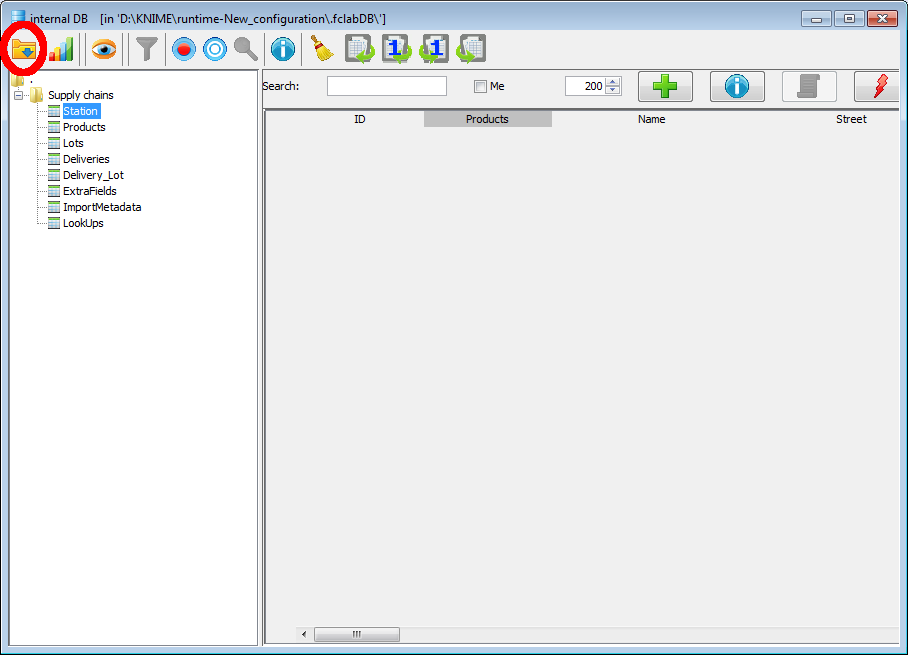
\includegraphics[height=0.6\textheight]{5.png}
	\end{center}
	\begin{itemize}
		\item
	\end{itemize}
\end{frame}

\subsection{6}
\begin{frame}
	\begin{center}
  		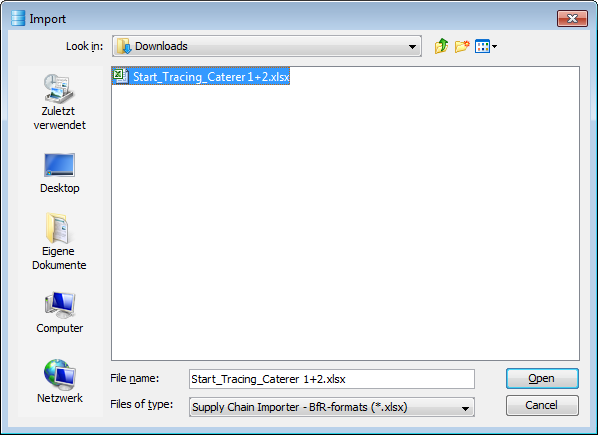
\includegraphics[height=0.5\textheight]{6.png}
	\end{center}
	\begin{itemize}
		\item
	\end{itemize}
\end{frame}

\subsection{7}
\begin{frame}
	\begin{center}
  		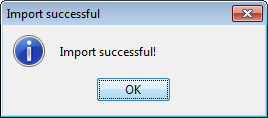
\includegraphics[width=0.4\textwidth]{7.png}
	\end{center}
	\begin{itemize}
		\item
	\end{itemize}
\end{frame}

\subsection{8}
\begin{frame}
	\begin{center}
  		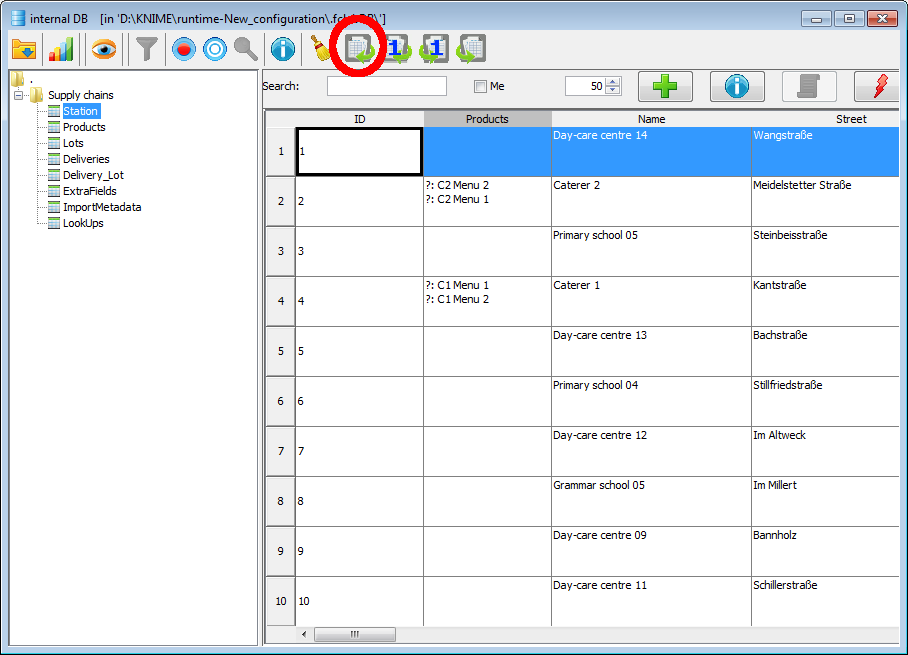
\includegraphics[height=0.6\textheight]{8.png}
	\end{center}
	\begin{itemize}
		\item
	\end{itemize}
\end{frame}

\subsection{9}
\begin{frame}
	\begin{center}
  		
\includegraphics[width=0.4\textwidth]{9.png}
	\end{center}
	\begin{itemize}
		\item
	\end{itemize}
\end{frame}

\subsection{10}
\begin{frame}
	\begin{center}
  		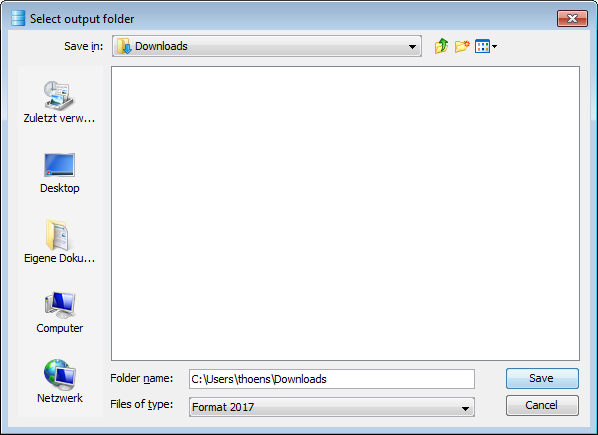
\includegraphics[height=0.5\textheight]{10.png}
	\end{center}
	\begin{itemize}
		\item
	\end{itemize}
\end{frame}

\subsection{11}
\begin{frame}
	\begin{center}
  		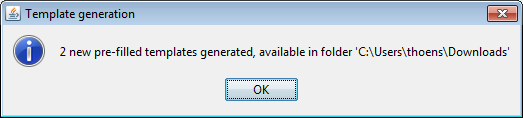
\includegraphics[width=0.8\textwidth]{11.png}
	\end{center}
	\begin{itemize}
		\item
	\end{itemize}
\end{frame}

\subsection{12}
\begin{frame}
	\begin{center}
  		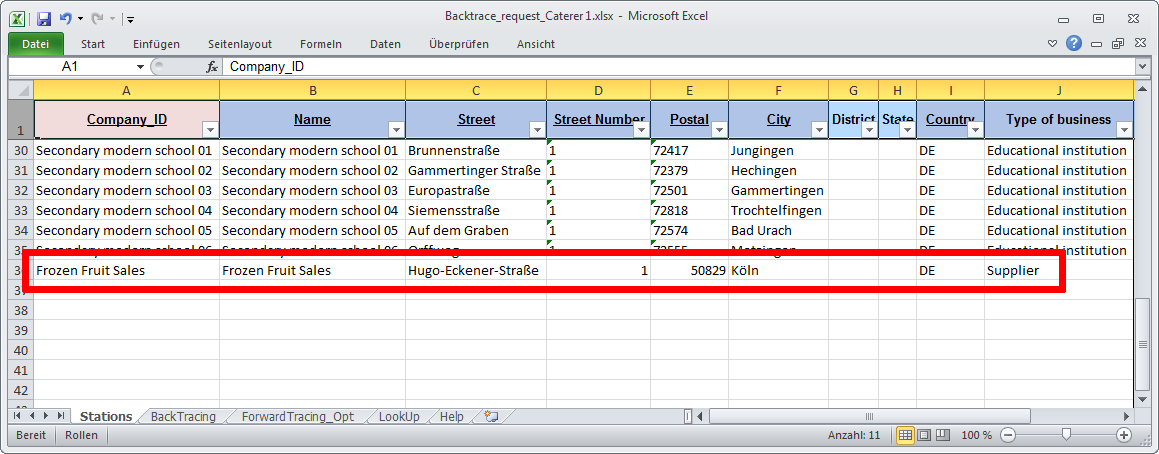
\includegraphics[width=0.95\textwidth]{12.png}
	\end{center}
	\begin{itemize}
		\item
	\end{itemize}
\end{frame}

\subsection{13}
\begin{frame}
	\begin{center}
  		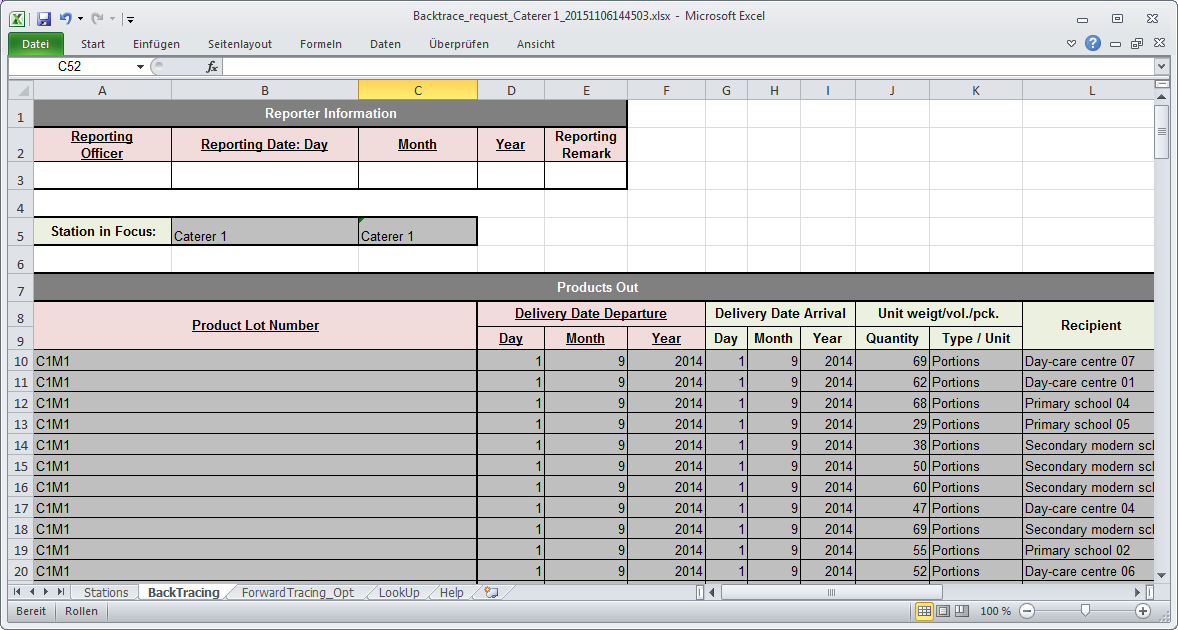
\includegraphics[width=0.95\textwidth]{13.png}
	\end{center}
	\begin{itemize}
		\item
	\end{itemize}
\end{frame}

\subsection{14}
\begin{frame}
	\begin{center}
  		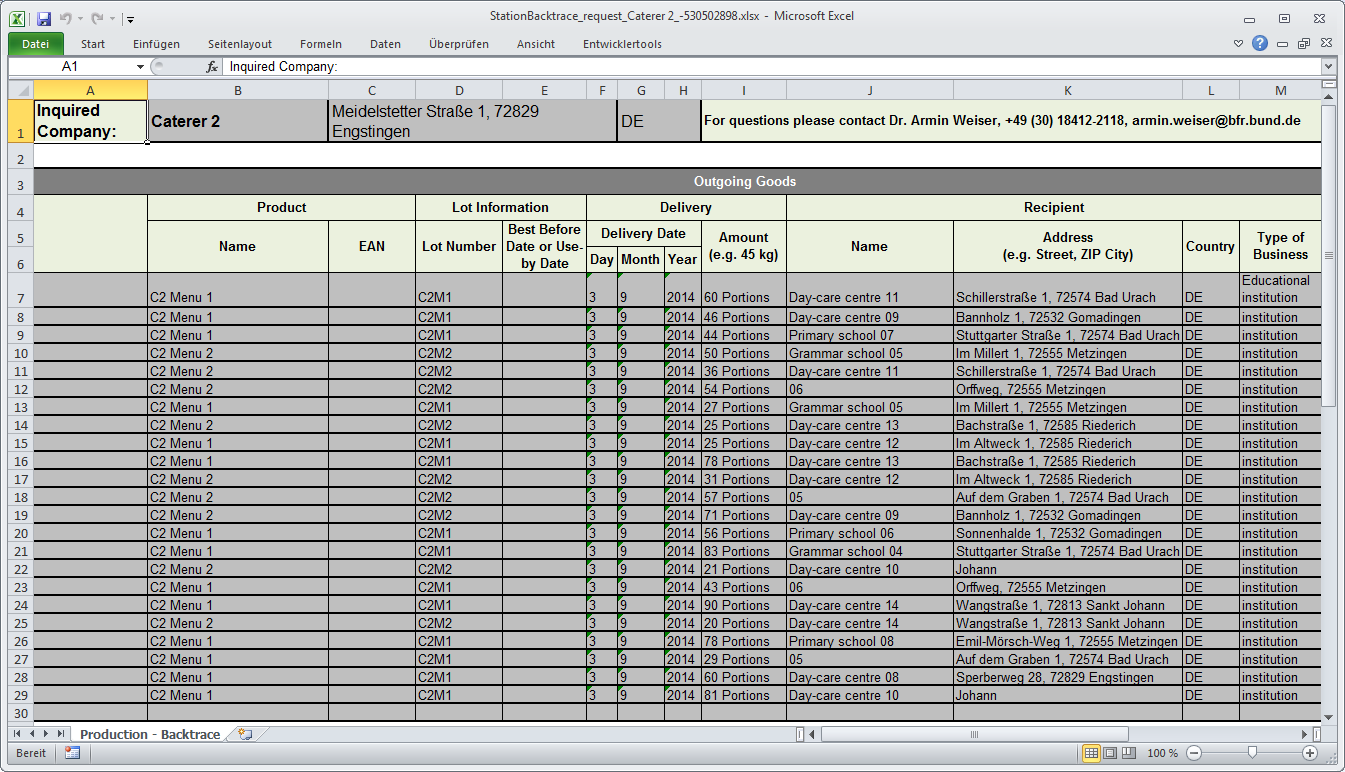
\includegraphics[width=0.95\textwidth]{14.png}
	\end{center}
	\begin{itemize}
		\item
	\end{itemize}
\end{frame}

\subsection{15}
\begin{frame}
	\begin{center}
  		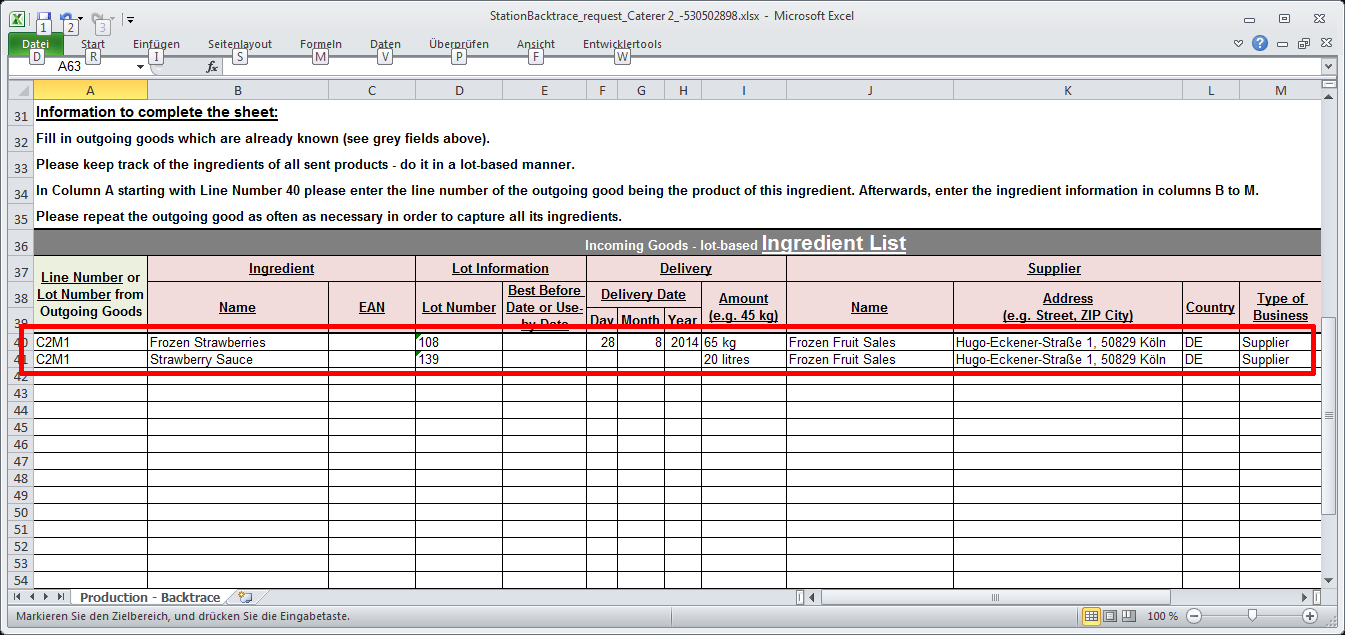
\includegraphics[width=0.95\textwidth]{15.png}
	\end{center}
	\begin{itemize}
		\item
	\end{itemize}
\end{frame}

\subsection{16}
\begin{frame}
	\begin{center}
  		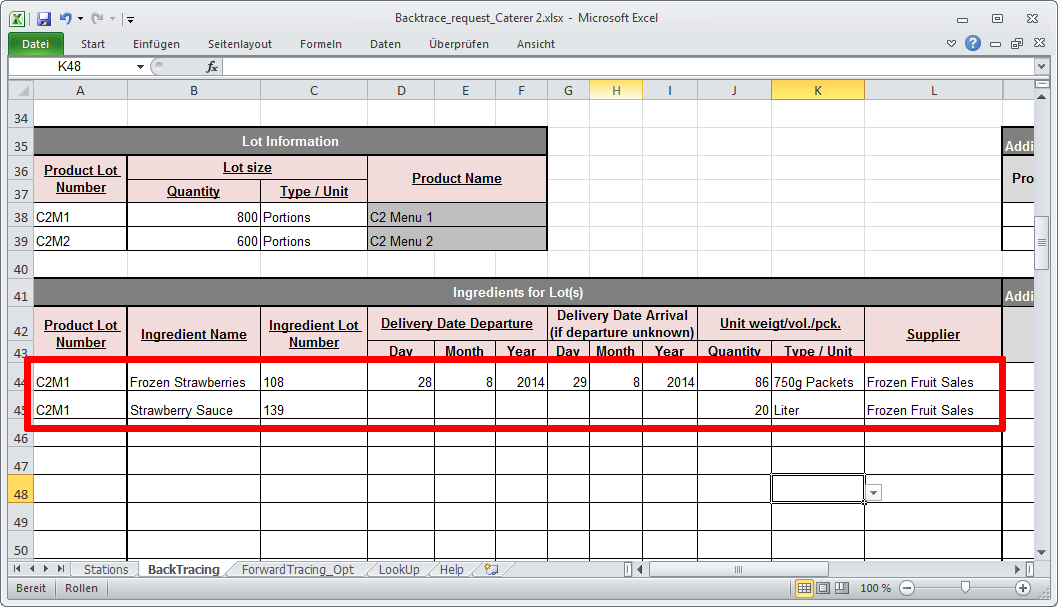
\includegraphics[width=0.95\textwidth]{16.png}
	\end{center}
	\begin{itemize}
		\item
	\end{itemize}
\end{frame}

\subsection{17}
\begin{frame}
	\begin{center}
  		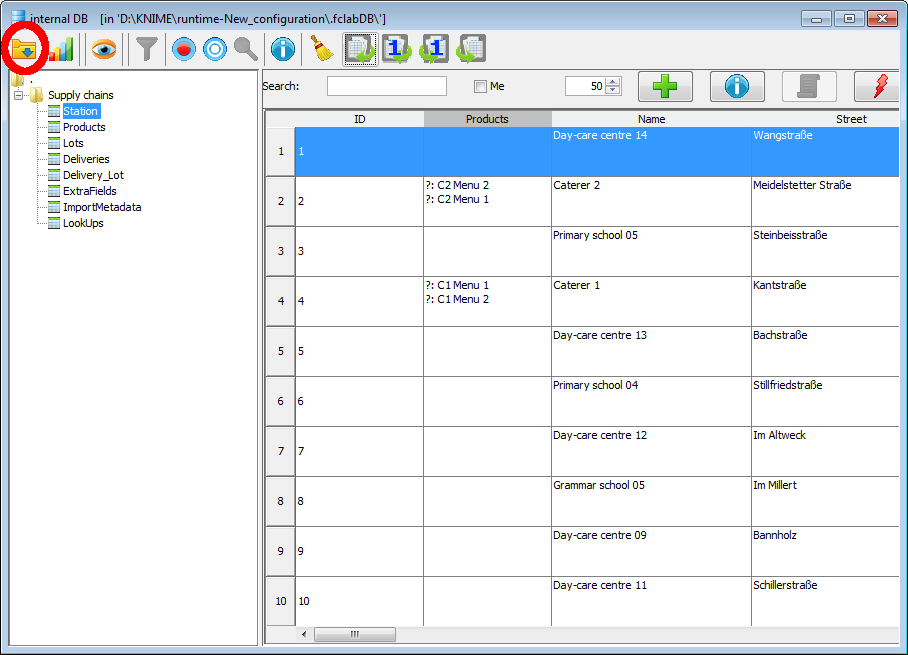
\includegraphics[height=0.6\textheight]{17.png}
	\end{center}
	\begin{itemize}
		\item
	\end{itemize}
\end{frame}

\subsection{18}
\begin{frame}
	\begin{center}
  		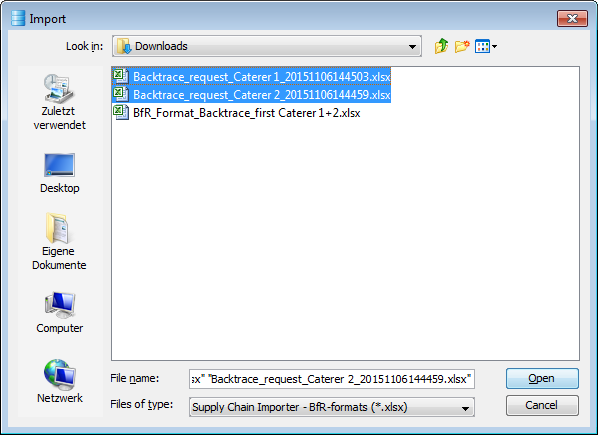
\includegraphics[height=0.5\textheight]{18.png}
	\end{center}
	\begin{itemize}
		\item
	\end{itemize}
\end{frame}

\subsection{19}
\begin{frame}
	\begin{center}
  		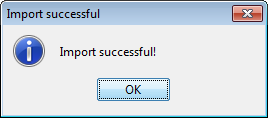
\includegraphics[width=0.4\textwidth]{19.png}
	\end{center}
	\begin{itemize}
		\item
	\end{itemize}
\end{frame}

\end{document}